\chapter{Hunter: Tracing Anycast}
\label{ch:hunter}

As discussed in previous chapters, anycast infrastructures introduce significant challenges regarding geographic transparency and control over Internet communications. Since multiple geographically distributed servers share the same IP address, determining the actual physical destination of a communication becomes substantially more complex than in traditional unicast environments. Routing decisions depend on dynamic BGP policies, peering relationships, traffic engineering mechanisms, and network conditions, making the geographic behavior of anycast communications difficult to predict and verify.

This lack of geographic determinism has direct implications for privacy, data protection, and data sovereignty. In particular, organizations and users may be unable to determine whether personal data remain within specific jurisdictions or are unintentionally transferred across national borders. Consequently, understanding the actual geographic destinations reached by anycast communications becomes a fundamental requirement for evaluating compliance with modern data protection regulations.

However, identifying the physical destination of anycast communications is a non-trivial problem. Traditional IP geolocation databases are insufficient in this context because a single anycast IP address may correspond to multiple geographically distributed replicas. Furthermore, the destination reached by a communication may dynamically vary depending on the origin network and current routing conditions.

To address these challenges, this chapter presents a methodology capable of inferring the potential geographic destinations of anycast communications from a given origin network. The proposed approach combines active network measurements, traceroute analysis, latency estimation, and multilateration techniques to estimate the physical regions where anycast replicas are likely deployed.

Based on this methodology, an automated framework named Hunter was developed to enable large-scale analysis of anycast infrastructures. Hunter performs distributed measurements from multiple vantage points, identifies routing paths towards anycast destinations, estimates geographic constraints using latency measurements, and ultimately determines the most likely destination countries associated with the communication.

The proposed methodology is composed of three sequential stages. First, the routing path towards the anycast destination is analyzed in order to identify the network elements traversed by the communication. Particular attention is devoted to the last observable hop before reaching the destination, as this network element provides critical information regarding the possible location of the anycast replica.

Second, multilateration techniques are applied using geographically distributed vantage points located near the last observable hop. By combining latency measurements from multiple probes, the methodology estimates the geographic region where the destination infrastructure is likely deployed.

Finally, the obtained region is analyzed to infer the corresponding city and country associated with the communication destination. When executed through Hunter, the methodology outputs the most likely geographic destination of the anycast communication or returns an indeterminate result if sufficient confidence cannot be achieved.

Figure~\ref{fig:hunter_steps} summarizes the different stages of the Hunter methodology.

\begin{figure}
    \centering
    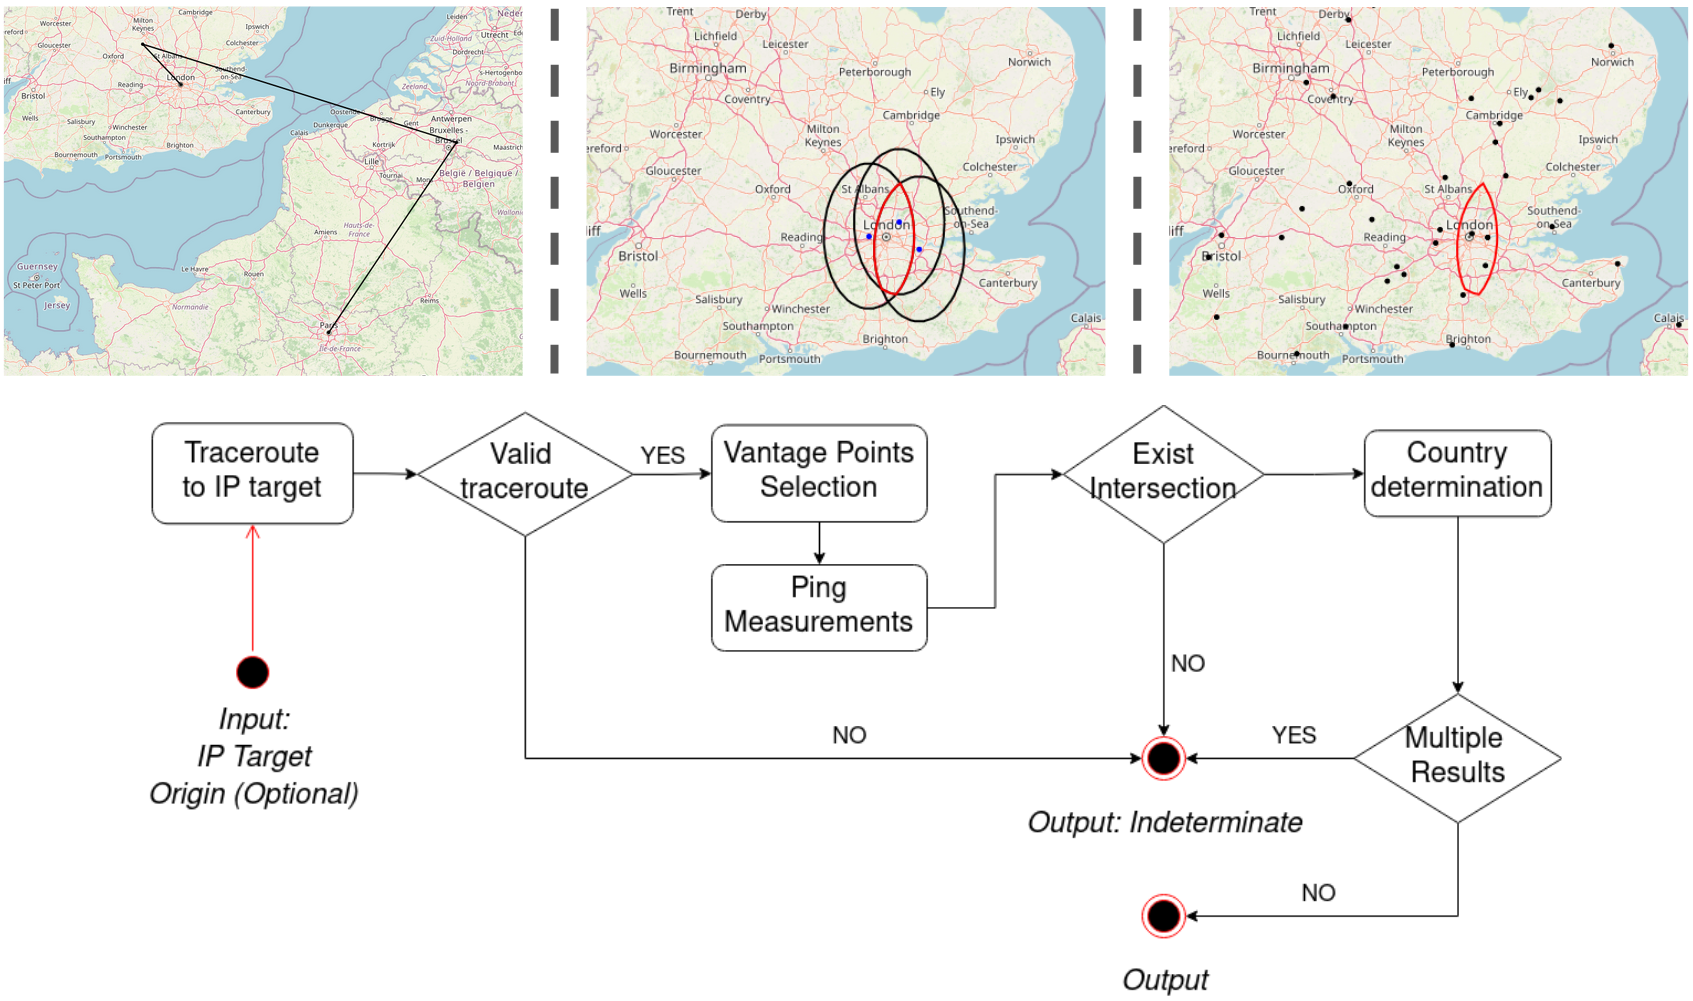
\includegraphics[width=\textwidth]{figures/hunter_steps.png}
    \caption{Hunter methodology for determining the destination country of anycast communications.}
    \label{fig:hunter_steps}
\end{figure}

The remainder of this chapter is organized as follows. Section~\ref{sc:hunter_tracing_path} presents the traceroute-based path analysis methodology. Afterwards, the multilateration process and geographic inference techniques are described. Finally, the Hunter implementation and its limitations are discussed.

\section{Tracing the Anycast Path}
\label{sc:hunter_tracing_path}

\subsection{Problem Definition}

The first step required to estimate the geographic destination of an anycast communication consists of analyzing the routing path followed by packets towards the target infrastructure. Unlike traditional unicast services, anycast destinations may correspond to multiple geographically distributed replicas sharing the same IP address. Consequently, identifying the physical destination reached by a communication requires inferring which replica is effectively serving the traffic from a given origin network.

A direct geolocation of the anycast IP address is generally insufficient for this purpose. Commercial geolocation databases typically associate a single geographic location with each IP address, while anycast infrastructures may simultaneously operate replicas across multiple regions or countries. Furthermore, the geographic destination reached by a communication may dynamically vary according to BGP routing policies, traffic engineering decisions, or network conditions.

To address this problem, Hunter analyzes the routing path towards the anycast destination using traceroute-based measurements. The objective of this phase is not to fully reconstruct the end-to-end topology, but rather to identify the network elements closest to the actual destination infrastructure. In particular, the methodology focuses on determining the last observable hop before the anycast replica, since this router provides valuable information regarding the geographic region where the destination is likely deployed.

\subsection{Traceroute-Based Path Analysis}

Hunter relies on traceroute measurements to analyze the path followed by packets towards the anycast destination. Traceroute operates by sending packets with progressively increasing Time-To-Live (TTL) values, forcing intermediate routers to generate ICMP ``Time Exceeded'' responses when the TTL reaches zero. By collecting these responses, traceroute reveals the sequence of routers traversed by the communication path.

For each target anycast IP address, traceroute measurements are executed from distributed RIPE Atlas probes located in different geographic regions. Using geographically diverse vantage points is essential because anycast routing decisions depend on the origin network of the communication. Different probes may therefore reach different replicas of the same anycast service.

The obtained traceroute paths are analyzed to identify stable routing patterns and determine the routers located closest to the destination infrastructure. Since routing paths may vary over time due to dynamic BGP updates or traffic engineering mechanisms, Hunter performs repeated measurements in order to reduce the impact of transient routing changes.

\subsection{Last Observable Hop Identification}

One of the key assumptions of the proposed methodology is that the last observable hop before the anycast destination is topologically close to the actual serving replica. Although the destination server itself may not respond to traceroute probes, nearby routers often generate ICMP responses that can be observed during the measurement process.

Hunter therefore identifies the last responsive router appearing before the destination IP address in the traceroute path. This router is referred to as the \textit{last observable hop}. Figure~\ref{fig:last_hop_example} illustrates this concept.

\begin{figure}
    \centering
    \includegraphics[width=\textwidth]{figures/last_hop_example.png}
    \caption{Example of traceroute path analysis and identification of the last observable hop before the anycast destination.}
    \label{fig:last_hop_example}
\end{figure}

The last observable hop constitutes the primary reference point used by Hunter to estimate the geographic region associated with the anycast destination. The rationale behind this approach is that routers located near the destination infrastructure are likely deployed within the same metropolitan area, Internet Exchange Point (IXP), or regional network environment.

However, this assumption introduces several limitations. In some cases, the last observable router may belong to a remote transit provider or may be located in a different city from the destination infrastructure. Additionally, MPLS tunnels, ICMP filtering, or hidden network segments may obscure parts of the routing path. These limitations are discussed later in this chapter.

\subsection{Selection of Measurement Vantage Points}

Once the last observable hop has been identified, Hunter selects nearby RIPE Atlas probes to perform additional latency measurements. The objective is to obtain geographically distributed measurements surrounding the estimated destination region.

The probe selection process considers both topological and geographic proximity. Probes located near the last observable hop are prioritized because they are more likely to reach the same anycast replica while minimizing the impact of long-distance routing asymmetries.

By combining measurements from multiple nearby vantage points, Hunter increases the accuracy of the subsequent multilateration phase and reduces the uncertainty associated with individual latency measurements.

\subsection{Path Stability and Measurement Validation}

Internet routing behavior is inherently dynamic. BGP updates, traffic engineering policies, congestion events, or failures may alter routing paths over time. Consequently, a single traceroute measurement may not accurately represent the long-term routing behavior of an anycast infrastructure.

To mitigate this issue, Hunter performs repeated measurements over time and compares the obtained paths in order to identify stable routing patterns. Measurements exhibiting substantial path instability or inconsistent routing behavior are discarded from the analysis.

Additionally, the methodology validates that selected RIPE Atlas probes consistently reach the same anycast region before including them in the multilateration stage. This validation step reduces the probability of mixing measurements associated with different anycast replicas.

\subsection{Limitations of Traceroute-Based Inference}

Although traceroute-based analysis provides valuable visibility into Internet routing behavior, several limitations affect the accuracy of path inference methodologies.

First, intermediate routers may filter ICMP responses or rate-limit traceroute packets, producing incomplete routing paths. Second, MPLS tunnels and hidden network segments may obscure portions of the topology. Third, routing asymmetries imply that the forward path observed by traceroute may differ from the reverse path followed by responses.

Additionally, anycast routing itself introduces extra complexity because routing decisions may dynamically change according to the origin network or temporal conditions. Consequently, different probes may observe substantially different paths towards the same destination IP address.

Despite these limitations, traceroute analysis remains one of the most effective techniques for inferring topological proximity to anycast infrastructures. Combined with distributed measurements and latency-based multilateration, it provides a practical foundation for estimating the geographic destination of anycast communications.

\section{Multilateration}
\label{sc:hunter_multilateration}

Once the last observable hop associated with the anycast communication has been identified, the next step consists of estimating the geographic region where the destination infrastructure is likely deployed. To achieve this objective, Hunter employs a multilateration-based methodology that combines latency measurements from geographically distributed RIPE Atlas probes.

The rationale behind this approach is based on the physical limitations imposed by signal propagation speed. Since network communications cannot travel faster than the speed of light, the measured Round Trip Time (RTT) between a probe and the destination provides an upper bound for the geographic distance separating them. By combining latency constraints obtained from multiple vantage points, it becomes possible to estimate the region where the destination infrastructure is likely located.

\subsection{Latency-Distance Estimation}

For each selected RIPE Atlas probe, Hunter performs ICMP ping measurements towards the last observable hop identified during the traceroute analysis phase. The minimum RTT observed across multiple measurements is used as the reference latency value, as it minimizes the impact of transient congestion, queuing delays, and routing variability.

Assuming an ideal propagation model, the theoretical maximum geographic distance associated with a measured RTT can be approximated according to the following relationship:

:contentReference[oaicite:0]{index=0}

where $d$ represents the maximum one-way geographic distance, $c$ corresponds to the signal propagation speed in the transmission medium, and $RTT$ denotes the measured round-trip time.

In practice, Internet communications do not follow geodesic paths and propagation speeds in optical fiber are lower than the speed of light in vacuum. Additionally, routing inefficiencies, switching delays, and intermediate processing introduce additional latency. Consequently, the obtained distance estimation should be interpreted as an upper bound rather than an exact geographic distance.

To account for these practical limitations, Hunter incorporates conservative propagation assumptions and tolerates moderate deviations between theoretical and observed distances.

\subsection{Probe Selection Strategy}

The accuracy of multilateration strongly depends on the geographic distribution of the selected probes. Hunter therefore prioritizes probes that satisfy two main conditions:

\begin{itemize}
    \item Geographic proximity to the estimated destination region.
    \item Stable routing behavior towards the same anycast replica.
\end{itemize}

The selection process begins with the probes previously identified during the tracing phase. Additional probes located within nearby geographic regions may also be incorporated to improve spatial coverage and reduce uncertainty.

Selecting probes located close to the destination region provides two important advantages. First, lower RTT measurements generally produce tighter geographic constraints. Second, nearby probes are more likely to reach the same anycast replica, reducing the probability of combining measurements associated with different destinations.

\subsection{Multilateration Process}

Once the latency measurements have been collected, Hunter applies multilateration techniques to estimate the geographic region satisfying all distance constraints simultaneously.

Each probe defines a circular geographic constraint centered at the probe location, where the radius corresponds to the maximum distance estimated from the RTT measurement. The destination infrastructure is expected to be located within the intersection region generated by all probes.

Figure~\ref{fig:multilateration_example} illustrates the multilateration process.

\begin{figure}
    \centering
    \includegraphics[width=\textwidth]{figures/multilateration_example.png}
    \caption{Example of multilateration using latency constraints from multiple RIPE Atlas probes.}
    \label{fig:multilateration_example}
\end{figure}

In ideal scenarios, the intersection of all regions converges into a relatively small geographic area, enabling Hunter to estimate the likely city or country associated with the anycast destination. However, due to measurement inaccuracies and routing variability, exact intersections may not always exist. In such cases, Hunter identifies the region minimizing the global inconsistency between all latency constraints.

\subsection{Geographic Inference}

After obtaining the multilateration region, Hunter maps the estimated area to geographic entities such as cities or countries. This process combines publicly available geographic datasets, RIPE Atlas probe metadata, and network infrastructure information.

The final objective of this phase is not to determine the exact coordinates of the anycast replica, but rather to identify the most likely jurisdiction where the communication is being processed. This distinction is particularly important from a regulatory perspective, since the primary concern of this thesis is determining whether communications remain within specific legal regions or cross international borders.

When the obtained multilateration region spans multiple countries or presents high uncertainty, Hunter classifies the result as indeterminate rather than forcing a potentially incorrect geographic attribution.

\subsection{Sources of Error and Limitations}

Several factors may affect the accuracy of latency-based multilateration.

First, Internet routing paths rarely follow geographically optimal routes. Traffic engineering policies, peering relationships, and operational constraints may introduce substantial detours that increase latency independently of geographic distance.

Second, RTT measurements may fluctuate due to congestion, queuing delays, or transient routing events. Although Hunter minimizes this effect by selecting minimum RTT values across repeated measurements, residual variability may still affect the estimation process.

Third, the propagation speed of optical signals depends on the physical transmission medium and network infrastructure characteristics. Consequently, the theoretical relationship between latency and distance constitutes only an approximation.

Finally, anycast infrastructures themselves introduce additional uncertainty because nearby probes may occasionally reach different replicas depending on routing dynamics. Hunter mitigates this issue through path validation and probe consistency checks performed during the tracing phase.

Despite these limitations, multilateration provides a practical and scalable mechanism for estimating the geographic regions associated with anycast communications. Combined with distributed traceroute analysis, it enables Hunter to infer likely destination jurisdictions with sufficient accuracy for large-scale privacy and compliance analyses.

\section{Country Determination}
\label{sc:hunter_country_determination}

The final stage of the Hunter methodology consists of determining the most likely country associated with the anycast communication. While the previous multilateration phase estimates a geographic region where the destination infrastructure is likely deployed, the objective of this stage is to translate that estimation into a jurisdictional context suitable for privacy and regulatory analyses.

This distinction is particularly important because the primary concern addressed by this thesis is not the precise physical location of a server, but rather whether communications remain within a specific legal region or cross international borders. Consequently, Hunter focuses on determining the country or jurisdiction associated with the destination infrastructure rather than attempting exact coordinate-level geolocation.

\subsection{Region Interpretation}

The multilateration phase produces an estimated geographic area representing the most likely region where the anycast replica is deployed. Depending on the quality and consistency of the latency measurements, this region may vary from a relatively small metropolitan area to a broader cross-border region.

Hunter interprets this multilateration output using geographic information systems and publicly available mapping datasets in order to determine the countries intersecting the estimated area. In scenarios where the inferred region is clearly contained within a single country, the attribution process is straightforward and the communication is associated with that jurisdiction.

However, the estimation process becomes more challenging when the multilateration region overlaps multiple countries or when the inferred area presents significant uncertainty. Such situations commonly occur near border regions, dense peering ecosystems, or highly interconnected metropolitan areas.

\subsection{Confidence-Based Country Attribution}

To improve reliability, Hunter applies a confidence-oriented attribution strategy rather than forcing deterministic classifications under uncertainty.

When the multilateration constraints consistently converge towards a specific geographic region and all candidate locations belong to the same country, Hunter classifies the destination as belonging to that jurisdiction with high confidence.

Conversely, when the estimated region spans multiple countries or when the measurements exhibit substantial inconsistencies, Hunter labels the result as indeterminate. This conservative approach minimizes the probability of introducing false geographic attributions that could compromise subsequent privacy or compliance analyses.

The methodology therefore prioritizes reliability over coverage. From the perspective of data protection analysis, an indeterminate result is preferable to an incorrect country assignment that may lead to inaccurate conclusions regarding cross-border data transfers.

\subsection{Integration of Auxiliary Information}

Although multilateration constitutes the primary geographic inference mechanism, Hunter also incorporates auxiliary information sources to improve the interpretation process.

These sources include:

\begin{itemize}
    \item RIPE Atlas probe metadata.
    \item Public routing information.
    \item Autonomous System (AS) ownership data.
    \item Internet Exchange Point (IXP) locations.
    \item Reverse DNS information when available.
\end{itemize}

Such information does not directly determine the destination country, but it provides contextual evidence that may help validate or reject candidate regions obtained during the multilateration phase.

For example, if the last observable hop belongs to an AS with infrastructure exclusively deployed within a specific country, this information may reinforce the plausibility of the corresponding multilateration result. Similarly, the presence of nearby IXPs or region-specific infrastructure may help explain observed routing behavior.

Nevertheless, Hunter avoids relying exclusively on administrative or declarative datasets because these sources are frequently incomplete, outdated, or insufficiently granular for accurately characterizing anycast infrastructures.

\subsection{Detection of Cross-Border Transfers}

Once the destination country has been determined, Hunter compares the inferred jurisdiction with the geographic origin associated with the communication or service under analysis.

If the destination country differs from the expected legal or geographic region, the communication is classified as a potential cross-border data transfer. This comparison enables Hunter to identify situations where user data may be routed towards foreign jurisdictions despite assumptions of regional confinement.

This capability is particularly relevant in the context of modern privacy regulations, where organizations are frequently required to disclose or restrict international transfers of personal data. By combining routing measurements with geographic inference, Hunter enables large-scale identification of potential discrepancies between expected and actual communication destinations.

\subsection{Sources of Uncertainty}

Country-level inference in anycast environments is inherently subject to uncertainty due to the dynamic nature of Internet routing and the limitations of network measurements.

Several factors may affect attribution accuracy:

\begin{itemize}
    \item Incomplete traceroute visibility.
    \item Latency fluctuations.
    \item Dynamic BGP routing changes.
    \item Routing asymmetries.
    \item Probe distribution limitations.
    \item Geographic proximity between neighboring countries.
\end{itemize}

Additionally, some anycast infrastructures intentionally deploy replicas near international borders or inside highly interconnected metropolitan regions where latency differences between countries are minimal. In such scenarios, distinguishing between neighboring jurisdictions using network measurements alone may be difficult.

Hunter explicitly accounts for these limitations by incorporating conservative confidence thresholds and supporting indeterminate classifications whenever sufficient certainty cannot be achieved.

\subsection{Final Output of Hunter}

After completing the tracing, multilateration, and country determination phases, Hunter produces a final geographic attribution associated with the analyzed anycast communication.

The output generated by the system may contain:

\begin{itemize}
    \item The inferred destination country.
    \item The estimated geographic region.
    \item The confidence level associated with the inference.
    \item Supporting routing and latency measurements.
    \item An indeterminate classification when reliable attribution is not possible.
\end{itemize}

This information enables subsequent large-scale analyses regarding geographic routing behavior, international data transfers, privacy policy compliance, and data sovereignty risks associated with anycast infrastructures.

\section{Validation Methodology}
\label{sc:hunter_validation}

Evaluating the accuracy of Hunter constitutes a challenging task due to the intrinsic characteristics of anycast infrastructures. Unlike traditional unicast services, anycast deployments typically do not publicly expose the exact geographic locations of their replicas. Furthermore, the destination reached by a communication may dynamically vary depending on the origin network and current routing conditions.

Consequently, validating the geographic inference methodology requires carefully selecting infrastructures for which reliable ground truth information can be obtained. This section describes the validation strategy followed to evaluate the accuracy and reliability of Hunter.

\subsection{Validation Objectives}

The validation process aims to evaluate several aspects of the proposed methodology:

\begin{itemize}
    \item The capability of Hunter to correctly infer the destination country associated with an anycast communication.
    \item The consistency of the inferred geographic regions across repeated measurements.
    \item The impact of routing dynamics and measurement variability on the obtained estimations.
    \item The robustness of the methodology under realistic Internet conditions.
\end{itemize}

The primary objective is not to achieve exact coordinate-level geolocation, but rather to determine whether Hunter can reliably identify the jurisdiction where communications are being processed. This distinction is particularly important because the ultimate goal of the methodology is to support privacy and compliance analyses involving international data transfers.

\subsection{Ground Truth Selection}

Obtaining reliable ground truth information for anycast infrastructures is inherently difficult because service providers rarely disclose the precise locations of their deployments. To mitigate this limitation, the validation process focuses on infrastructures whose geographic deployment can be independently verified.

The validation dataset includes infrastructures satisfying at least one of the following conditions:

\begin{itemize}
    \item Publicly documented anycast deployments.
    \item Services with regionally constrained infrastructures.
    \item Anycast deployments operated by organizations providing geographic transparency.
    \item Infrastructures whose locations can be corroborated through auxiliary information sources.
\end{itemize}

Additionally, the validation process incorporates manually verified measurements in which the inferred routing behavior can be contrasted against publicly available operational information, reverse DNS naming conventions, Internet Exchange Point (IXP) presence, or provider infrastructure documentation.

This approach does not completely eliminate uncertainty regarding the true destination of communications. However, it enables the construction of a sufficiently reliable validation framework for evaluating country-level inference accuracy.

\subsection{Measurement Procedure}

For each target anycast infrastructure, Hunter executes the complete methodology described in previous sections:

\begin{enumerate}
    \item Traceroute measurements are performed from distributed RIPE Atlas probes.
    \item The last observable hop before the anycast destination is identified.
    \item Additional latency measurements are collected from nearby probes.
    \item Multilateration is applied to estimate the likely destination region.
    \item The inferred region is mapped to a destination country.
\end{enumerate}

Measurements are repeated over time in order to reduce the impact of transient routing fluctuations and temporary network events. Repeated measurements also allow the methodology to evaluate the stability of the inferred destinations.

Whenever substantial routing inconsistencies are detected, the corresponding measurements are discarded from the validation dataset to avoid introducing unreliable inferences.

\subsection{Evaluation Metrics}

The performance of Hunter is evaluated using multiple complementary metrics.

\subsubsection{Country-Level Accuracy}

The primary evaluation metric is country-level accuracy, defined as the proportion of measurements for which Hunter correctly identifies the destination country associated with the anycast communication.

Country-level accuracy is particularly relevant from a regulatory perspective because modern privacy legislations generally operate at the jurisdictional level rather than at the city or coordinate level.

\subsubsection{Indeterminate Classification Rate}

Since Hunter adopts a conservative confidence-oriented strategy, some measurements may produce indeterminate results when sufficient certainty cannot be achieved.

The indeterminate classification rate measures the proportion of communications for which Hunter intentionally avoids assigning a country due to ambiguity or insufficient confidence.

This metric is important because it reflects the trade-off between coverage and reliability. A lower indeterminate rate increases coverage, but may also increase the probability of incorrect geographic attributions.

\subsubsection{Measurement Stability}

The validation process also evaluates the temporal stability of the inferred destinations. Repeated measurements are compared to determine whether Hunter consistently identifies the same geographic regions over time.

This metric provides insights regarding the sensitivity of the methodology to routing dynamics, congestion events, or transient topology changes.

\subsection{Sources of Error}

Several factors may affect the accuracy of the validation results.

First, anycast infrastructures may dynamically redirect traffic between replicas according to operational policies, congestion conditions, or failures. Consequently, the actual destination of a communication may legitimately change between measurements.

Second, traceroute measurements may provide incomplete visibility due to ICMP filtering, MPLS tunnels, or hidden network segments. These limitations may affect the identification of the last observable hop.

Third, latency-based multilateration inherently relies on approximations regarding signal propagation speed and routing efficiency. Real Internet paths rarely follow geographically optimal routes, potentially introducing deviations between estimated and actual distances.

Finally, the geographic distribution of RIPE Atlas probes is not uniform worldwide. Some regions exhibit dense probe coverage while others provide only limited measurement visibility. This imbalance may affect the precision of the inferred multilateration regions.

\subsection{Validation Limitations}

Although the proposed validation methodology provides meaningful insights regarding the performance of Hunter, several limitations must be acknowledged.

The first limitation is the absence of complete ground truth information for many commercial anycast infrastructures. In practice, it is often impossible to independently verify the precise geographic locations of all replicas associated with a service.

The second limitation is that Internet routing behavior is inherently dynamic. Consequently, validation results should be interpreted as representative observations rather than immutable properties of the analyzed infrastructures.

Additionally, the methodology focuses primarily on country-level inference accuracy. While city-level estimations may occasionally be obtained, the primary objective of Hunter is to support the analysis of cross-border data transfers and jurisdictional exposure.

Despite these limitations, the validation process demonstrates that Hunter provides sufficiently accurate and reliable geographic inferences for large-scale privacy and compliance analyses involving anycast infrastructures.

\section{Measurement Infrastructure}
\label{sc:hunter_measurement_platform}

The methodology proposed in Hunter requires performing distributed network measurements from geographically diverse vantage points. Although traceroute and latency measurements could theoretically be executed from a single host, such an approach would severely limit the geographic visibility of the inference process and would not adequately capture the routing diversity inherent to anycast systems.

To address this limitation, Hunter relies on RIPE Atlas \cite{HomeAtlas}, a large-scale Internet measurement platform composed of thousands of distributed probes deployed worldwide. RIPE Atlas enables researchers and network operators to execute active measurements such as ping, traceroute, DNS, TLS, HTTP, and NTP from multiple geographic and topological locations.

The distributed nature of RIPE Atlas is particularly relevant for anycast analysis because routing decisions in anycast systems strongly depend on the origin network of the communication. Consequently, measurements performed from geographically dispersed probes may reach different replicas of the same anycast infrastructure, providing visibility into the geographic distribution of the service.

RIPE Atlas probes are hosted by volunteers, Internet Service Providers (ISPs), research institutions, universities, and network operators. This broad deployment provides extensive visibility into the global Internet infrastructure and enables Internet-scale measurement studies across multiple countries and network environments.

The platform is publicly accessible and operates under a credit-based system that allows participants to contribute probes and execute measurements. RIPE Atlas is maintained by the RIPE Network Coordination Centre (RIPE NCC), the Regional Internet Registry responsible for Europe, the Middle East, and parts of Central Asia. Due to its operational maturity and widespread adoption within the network measurement community, RIPE Atlas has become one of the most widely used infrastructures for Internet-scale routing and performance analyses.

Several alternative measurement platforms exist, including Ark CAIDA \cite{ArkCAIDA}, perfSONAR \cite{PerfSONAR}, and PlanetLab \cite{HomePlanetLab}. However, RIPE Atlas was selected for this work due to four primary characteristics:

\begin{itemize}
    \item Large number of active probes.
    \item Extensive geographic distribution.
    \item Flexible measurement capabilities.
    \item Public API enabling automated large-scale measurements.
\end{itemize}

These characteristics are essential for Hunter because the methodology requires executing repeated traceroute and latency measurements from multiple distributed vantage points in order to estimate the geographic regions potentially reached by anycast communications.

\subsection{Probe Selection}

The selection of measurement probes constitutes a critical component of the Hunter methodology. Since anycast routing behavior depends on the origin network of the communication, different probes may reach different replicas of the same anycast infrastructure.

Hunter therefore selects probes according to both geographic and topological criteria. Initially, geographically distributed probes are used during the traceroute phase in order to identify candidate regions associated with the destination infrastructure. Subsequently, additional nearby probes are selected to perform latency measurements during the multilateration stage.

Priority is given to probes exhibiting stable connectivity, low measurement error rates, and consistent routing behavior. Measurements generated by unstable or intermittently connected probes are discarded in order to reduce inference uncertainty.

The framework additionally avoids combining measurements from probes reaching different anycast replicas, since this situation would invalidate the multilateration assumptions.

\subsection{Measurement Execution}

Hunter automates the execution of distributed measurements through the RIPE Atlas API. Traceroute and ping measurements are scheduled asynchronously in order to improve scalability and reduce execution time.

For each analyzed target, repeated measurements are performed over time to reduce the impact of transient routing fluctuations, temporary congestion events, or sporadic probe failures. Measurements producing incomplete routing paths or inconsistent latency observations are filtered during the data processing phase.

The framework additionally incorporates retry mechanisms and timeout management procedures to mitigate temporary operational issues associated with probe availability or RIPE Atlas rate limitations.

\subsection{Data Collection and Reproducibility}

All measurements executed by Hunter are automatically collected, normalized, and stored together with their associated metadata. This information includes routing paths, RTT observations, probe identifiers, timestamps, inferred regions, and confidence estimations.

Storing intermediate measurement results enables reproducibility and facilitates longitudinal analyses of routing behavior over time. Additionally, preserving the raw measurements allows the inference process to be independently re-evaluated under different assumptions or parameter configurations.

This capability is particularly important in anycast environments, where routing behavior may dynamically evolve according to operational policies, traffic engineering decisions, or infrastructure changes.

\section{Hunter Implementation}
\label{sc:hunter_implementation}

Based on the methodology described in the previous sections, an automated framework named Hunter was developed to enable large-scale inference of the geographic destinations associated with anycast communications. The implementation was designed with three primary objectives: scalability, reproducibility, and modularity.

Hunter automates the complete measurement and inference pipeline, including traceroute execution, last-hop identification, probe selection, latency collection, multilateration, and country inference. This automation is essential to support Internet-scale analyses involving thousands of anycast communications and distributed measurement probes.

\subsection{System Architecture}

Hunter follows a modular pipeline architecture in which each stage of the methodology is implemented as an independent processing component. Figure~\ref{fig:hunter_architecture} presents an overview of the system architecture.

\begin{figure}
    \centering
    \includegraphics[width=\textwidth]{figures/hunter_architecture.png}
    \caption{High-level architecture of the Hunter framework.}
    \label{fig:hunter_architecture}
\end{figure}

The framework receives as input a target anycast IP address or domain name. If a domain name is provided, the corresponding DNS resolution process is first executed in order to obtain the associated anycast IP addresses.

Once the target has been identified, Hunter coordinates distributed traceroute measurements using RIPE Atlas probes. The obtained routing paths are then processed to identify the last observable hop associated with the destination infrastructure.

Subsequently, nearby probes are selected to perform additional latency measurements towards the identified region. The collected RTT measurements are processed by the multilateration engine, which estimates the geographic region likely associated with the destination infrastructure. Finally, the country inference module determines the most probable jurisdiction corresponding to the communication destination.

\subsection{Measurement Orchestration}

Hunter relies on the RIPE Atlas API to execute and manage distributed measurements. The framework automates the complete lifecycle of the measurement process, including probe selection, measurement scheduling, result collection, and failure handling.

Traceroute and ping measurements are executed asynchronously in order to reduce execution time and improve scalability. Since Internet-scale analyses may require thousands of measurements, asynchronous orchestration significantly reduces the time needed to complete the inference process.

The framework also incorporates retry mechanisms to mitigate temporary failures caused by unavailable probes, transient connectivity issues, or RIPE Atlas rate limitations. Measurements producing incomplete or inconsistent results are discarded to avoid introducing unreliable inferences.

\subsection{Data Processing Pipeline}

The data processing pipeline is responsible for extracting relevant information from the raw measurements returned by RIPE Atlas.

For traceroute measurements, Hunter parses the sequence of observed hops and identifies the last responsive router appearing before the destination. The framework additionally filters incomplete paths, inconsistent traces, and anomalous measurements that may negatively affect the inference process.

For latency measurements, the framework aggregates repeated RTT samples and selects the minimum observed latency value as the reference metric. This strategy minimizes the impact of transient congestion, queuing delays, and temporary routing variability.

The processed measurements are then normalized and passed to the multilateration engine for geographic estimation.

\subsection{Geographic Inference Engine}

The geographic inference engine constitutes the core analytical component of Hunter. This module combines the latency constraints obtained from distributed probes in order to estimate the most likely geographic region associated with the anycast destination.

The engine applies multilateration techniques to determine the region minimizing the global inconsistency among all latency-derived distance constraints. Once the candidate region has been estimated, Hunter maps the result to geographic entities such as metropolitan areas or countries.

The framework additionally incorporates confidence estimation mechanisms to determine whether the obtained inference is sufficiently reliable. When the uncertainty associated with the estimation exceeds predefined thresholds, Hunter classifies the result as indeterminate instead of forcing a potentially incorrect attribution.

\subsection{Automation and Scalability}

One of the primary design goals of Hunter was supporting large-scale Internet measurements. Consequently, the framework was developed to operate in a fully automated manner with minimal manual intervention.

The modular architecture allows measurements, path analysis, multilateration, and geographic inference to be executed independently and in parallel. This design significantly improves scalability and enables Hunter to process large datasets involving thousands of destinations and distributed probes.

Additionally, the framework stores intermediate measurement results and metadata, enabling reproducibility and facilitating subsequent analyses. This capability is particularly relevant for longitudinal studies, where repeated measurements may be compared over time in order to evaluate routing stability or geographic variability.

\section{Validation Results}
\label{sc:hunter_validation_results}

After implementing the complete Hunter framework, the proposed methodology was evaluated in order to determine its capability to correctly infer the geographic destinations associated with anycast communications.

The objective of this validation process is not to demonstrate exact coordinate-level geolocation accuracy, but rather to evaluate whether Hunter can reliably identify the destination jurisdictions associated with anycast infrastructures.

\subsection{Validation Dataset}

The validation dataset was composed of anycast infrastructures for which sufficiently reliable geographic information could be independently verified. The selected services included infrastructures with publicly documented deployments, regionally constrained services, and infrastructures whose locations could be corroborated using auxiliary routing and operational information.

Measurements were performed from geographically distributed RIPE Atlas probes covering multiple countries and network environments. Repeated measurements were executed over time in order to reduce the impact of transient routing fluctuations and temporary network events.

\subsection{Country-Level Accuracy}

The primary evaluation metric used in this work is country-level inference accuracy. The validation process demonstrated that Hunter is capable of correctly identifying the destination jurisdiction for a substantial proportion of the analyzed communications.

The obtained results indicate that combining traceroute analysis, distributed latency measurements, and multilateration techniques provides sufficient information to infer the likely destination country of many anycast communications.

The accuracy of the methodology strongly depends on several factors, including probe density, routing stability, visibility of intermediate routers, and geographic separation between candidate regions.

\subsection{Temporal Stability}

To evaluate the robustness of the methodology, repeated measurements were performed over time towards the same anycast infrastructures.

The obtained results showed that stable infrastructures generally produced consistent geographic inferences across repeated executions. However, certain anycast deployments exhibited dynamic routing behavior, occasionally redirecting traffic towards different replicas depending on network conditions or routing policies.

These observations highlight the dynamic nature of anycast systems and reinforce the importance of repeated measurements when analyzing geographic routing behavior.

\subsection{Indeterminate Results}

Hunter intentionally adopts a conservative inference strategy in order to reduce the probability of incorrect geographic attributions.

Consequently, some measurements produced indeterminate results when the multilateration region overlapped multiple countries or when the obtained measurements presented substantial inconsistencies.

Although this strategy reduces total coverage, it significantly improves the reliability of the final geographic attributions and minimizes the risk of false positive country assignments.

\subsection{Error Analysis}

The validation process additionally revealed several sources of error affecting geographic inference accuracy.

The most relevant limitations include incomplete traceroute visibility due to ICMP filtering, MPLS tunnels hiding portions of the routing path, routing asymmetries, and dynamic BGP routing changes.

Additionally, regions with sparse RIPE Atlas probe coverage presented larger multilateration uncertainty due to the reduced number of nearby vantage points.

Despite these limitations, the obtained results demonstrate that Hunter provides sufficiently accurate country-level inferences to support large-scale analyses regarding international data transfers and geographic routing behavior.

\section{Limitations}
\label{sc:hunter_limitations}

Although Hunter provides a practical and scalable methodology for inferring the geographic destinations of anycast communications, several limitations must be acknowledged.

\subsection{Routing Visibility Limitations}

Hunter relies heavily on traceroute measurements to infer topological proximity to the destination infrastructure. However, Internet routing visibility is inherently incomplete.

Intermediate routers may filter ICMP responses, apply rate limiting policies, or hide portions of the routing path through MPLS tunnels or internal network mechanisms. Consequently, the last observable hop identified by Hunter may not always correspond to the router physically closest to the destination infrastructure.

\subsection{Dynamic Anycast Routing}

Anycast routing behavior is inherently dynamic. Traffic engineering policies, congestion events, routing changes, or failures may cause communications to be redirected towards different replicas over time.

As a result, repeated measurements from the same origin network may occasionally reach different geographic destinations. Although Hunter mitigates this issue through repeated measurements and path validation mechanisms, routing dynamics remain an intrinsic limitation of anycast inference methodologies.

\subsection{Probe Distribution Constraints}

The accuracy of multilateration strongly depends on the geographic distribution of available measurement probes.

Regions with dense RIPE Atlas coverage generally produce more accurate estimations due to the availability of multiple nearby vantage points. Conversely, areas with sparse probe deployment may exhibit larger uncertainty regions and reduced inference precision.

This limitation is particularly relevant in regions with limited Internet measurement infrastructure or reduced participation in community-driven measurement platforms.

\subsection{Latency-Based Estimation Limitations}

Hunter estimates geographic constraints using RTT measurements. However, Internet routing paths rarely follow geographically optimal routes.

Traffic engineering decisions, peering relationships, and operational constraints may introduce significant routing detours that increase latency independently of physical distance. Consequently, the relationship between RTT and geographic distance should be interpreted as an approximation rather than an exact mapping.

Additionally, transient congestion and queuing delays may introduce variability into latency measurements despite the filtering strategies employed by the framework.

\subsection{Jurisdictional Granularity}

The primary objective of Hunter is to determine the country or jurisdiction associated with an anycast communication rather than the exact geographic coordinates of the destination infrastructure.

While city-level estimations may occasionally be obtained, the methodology is specifically optimized for identifying potential cross-border communications and supporting privacy and compliance analyses.

Therefore, Hunter should not be interpreted as a precise IP geolocation system, but rather as a geographic inference framework designed for jurisdictional analysis in distributed anycast environments.

\section{Chapter Summary}
\label{sc:hunter_summary}

This chapter presented Hunter, a methodology and automated framework designed to infer the geographic destinations associated with anycast communications.

The chapter first introduced the challenges associated with geographic inference in anycast environments and described the proposed methodology based on distributed traceroute analysis, last-hop identification, latency-based multilateration, and country inference.

Afterwards, the validation methodology and the obtained validation results were presented, demonstrating that Hunter provides sufficiently reliable country-level inferences for analyzing international data transfers and geographic routing behavior.

The chapter additionally described the distributed measurement infrastructure and the implementation details of the Hunter framework, emphasizing its scalability, modularity, and automation capabilities.

Finally, the main limitations affecting anycast inference methodologies were discussed, including routing visibility constraints, probe distribution limitations, and the dynamic nature of anycast routing.

The following chapter leverages Hunter to conduct large-scale analyses of anycast-based communications in real-world environments, focusing on privacy risks, international data transfers, and geographic transparency within the Android ecosystem.
```
